\section*{Problem 5}
	\begin{proof} [Solution]
		I choose the following list:
		\begin{itemize}
			\item Animal Farm by George Orwell
			\item Harry Potter and the Sorcerer\textquotesingle s Stone by Joanne Kathleen Rowling
			\item Romeo and Juliet by William Shakespeare
			\item The Adventures of Sherlock Holmes by Arthur Conan Doyle
			\item The Fellowship of the Ring by John Ronald Reuel Tolkien
		\end{itemize}
		Here is the result. We can see that the ratio analysis is sufficiently effective for the comparision.
		\begin{center}
			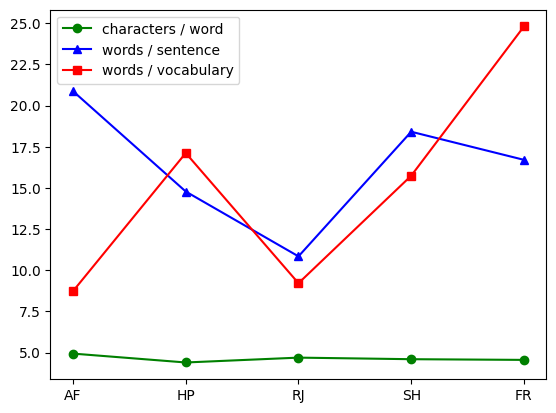
\includegraphics[width=0.5\textwidth]{words.png}
		\end{center}
		For this comparision, we can think about:
		\begin{itemize}
			\item Vocabulary and Grammar: Specific word choice, complexity of sentence structure, and use of sentence types
			\item Point of view and narrator: First-person and third-person, differences in narrative structure
			\item Literary techniques: various literary expression methods including metaphor, irony, etc.
			\item Morphemes: Frequency of use in words containing adverbs and adjectives
		\end{itemize}
	\end{proof}